\documentclass[border=2pt]{standalone}
\usepackage{tikz}

\begin{document}
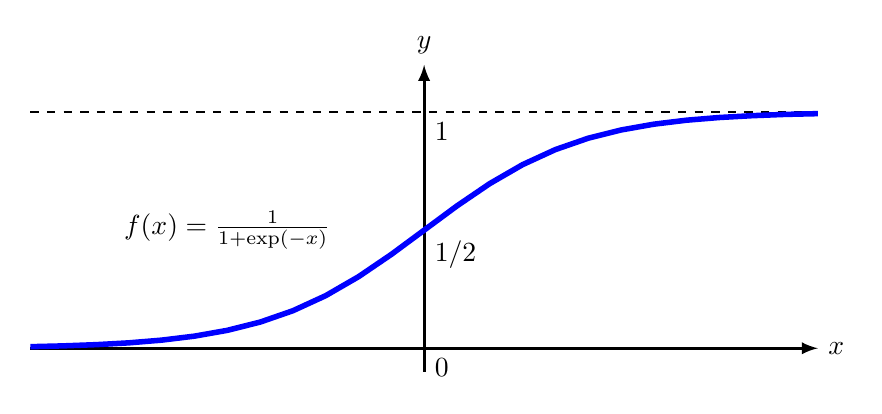
\begin{tikzpicture}[yscale=3, line width=1pt]
    \draw [-latex] (-5, 0) -- (5, 0) node[right] {$ x $};
    \draw [-latex] (0, -0.1) -- (0, 1.2) node[above] {$ y $};

    \draw[dashed] (-5, 1) -- (5, 1);
    \draw[blue, line width=2pt, domain=-5:5, variable=\x] plot({\x}, {1/(1+exp(-\x))});

    \node at (-2.5, 0.5) {$ f(x) = \frac{1}{1 + \exp (-x)} $};

    \node [below right] at (0, 0) {$ 0 $};
    \node [below right] at (0, 0.5) {$ 1/2 $};
    \node [below right] at (0, 1) {$ 1 $};

\end{tikzpicture}
\end{document}